\subsection{Строковые абстрактные домены}

Пример простого строкового абстрактного домена реализован в системе \textbf{JSAI} --- платформе статического анализа JavaScript ~\cite{guha2012jsai}. В ней строки представляются в виде:
\begin{itemize}
    \item любая ($\top$) и неинициализированная ($\bot$) строки
    \item константные строки
    \item категории ``строка-число'', ``спец-символ'' и ``любая строка''
\end{itemize}

\begin{figure}[H]
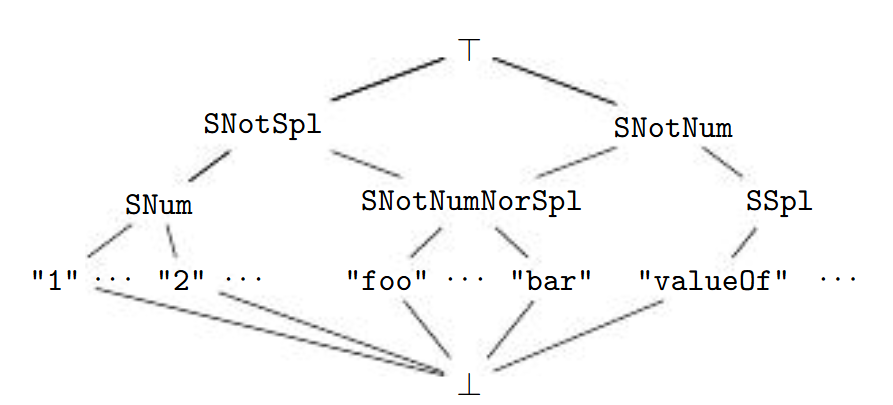
\includegraphics[width=\textwidth]{images/jsai-string-lattice.png}\hfill
\end{figure}


Хотя этот подход обладает высокой производительностью, он страдает от недостатка точности. Например, пусть переменная $s$ может быть равна строке ``foo'' или ``bark''. Тогда значение выражения \texttt{s.length} может быть либо $3$, либо $4$, но абстрактный домен JSAI вернёт «любая длина». Это делает невозможным отбрасывание условий вроде \texttt{if (s.length == 0)} как недостижимых, что ведёт к ложным срабатываниям

\newpage
\begin{lstlisting}[caption={Пример недостаточной точности в строковом домене JSAI}]
let s;
if (input == 0) {
    s = "foo";
} else {
    s = "bark";
}
if (s.length == 0) {
    throw new Error("Divide by zero!");
}
let repeats = 100 / str.length;
\end{lstlisting}




\newpage
\subsection{Уточнение анализа с помощью конечных автоматов}

Для повышения точности анализа был предложен подход, основанный на \textbf{конечных автоматах с переходами по буквам}, описанный в работе~\cite{apinis2020symbolic}. В этом подходе множество возможных значений строк моделируется как язык, распознаваемый конечным автоматом. Операции над строками соответствуют операциям над языками: объединение, пересечение, конкатенация и пр.

\subsubsection*{Преимущества}
\begin{itemize}
    \item высокая точность
\end{itemize}

\subsubsection*{Недостатки}
\begin{itemize}
    \item высокая вычислительная сложность
    \item большое потребление памяти
    \item низкая масштабируемость при анализе больших программ
\end{itemize}

\begin{figure}[h]
    \centering
    \begin{tikzpicture}[shorten >=1pt,node distance=1.8cm,on grid,auto]
        \node[state,initial] (q0) {$q_0$};
        \node[state] (q1) [right of=q0] {$q_1$};
        \node[state] (q2) [right of=q1] {$q_2$};
        \node[state,accepting] (q3) [right of=q2] {$q_3$};

        \node[state] (p1) [below of=q1] {$p_1$};
        \node[state] (p2) [right of=p1] {$p_2$};
        \node[state] (p3) [right of=p2] {$p_3$};
        \node[state,accepting] (p4) [right of=p3] {$p_4$};

        \path[->]
          (q0) edge node {f} (q1)
          (q1) edge node {o} (q2)
          (q2) edge node {o} (q3)

          (q0) edge[bend right] node {b} (p1)
          (p1) edge node {a} (p2)
          (p2) edge node {r} (p3)
          (p3) edge node {k} (p4);
    \end{tikzpicture}
    \caption{Конечный автомат, распознающий строки ``foo'' и ``bark''}
\label{fig:automaton}
\end{figure}

Овер-аппроксимация строк в конечных автоматах повышает точность анализа строк во многих сценариях, но она не подходит для реальных программ, работающих со статически неизвестными входными данными и манипуляциями с длинным текстом




\newpage
\subsection{TARSIS}

TARSIS (Template-based Abstract Representation of Strings with Static analysis) — это современный строковый абстрактный домен, предложенный в работе~\cite{tarsis2021}. Основное новшество Tarsis заключается в том, что он работает с алфавитом строк, а не с отдельными символами. С одной стороны, такой подход требует более сложного и уточненного определения расширяющего оператора и абстрактной семантики строковых операторов. С другой стороны, это позволяет получать более точные результаты

\subsubsection*{Основные функции}
В статье описан алгоритм для аппроксимации с доказательством полноты наиболее часто использующихся функций на строках, а именно substr, length, indexOf, replace, concat и contains

\begin{figure}[H]
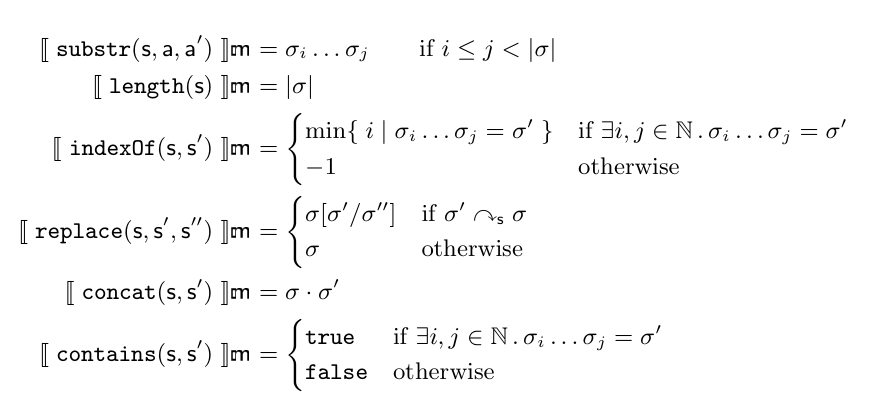
\includegraphics[width=\textwidth]{images/tarsis-functions.png}\hfill
\end{figure}

\newpage
\subsubsection*{Widening}
Важным методом аппроксимации является widening. Именно благодаря ему удается завершать циклы за конечное время, создавая аппроксимацию. Рассмотрим пример того, как это реализованно

\begin{lstlisting}[caption={Пример применения widening}]
function f(v) {
    res = "";
    while(?) res = res + "id = " + v;
    return res;
}
\end{lstlisting}

\begin{figure}[H]
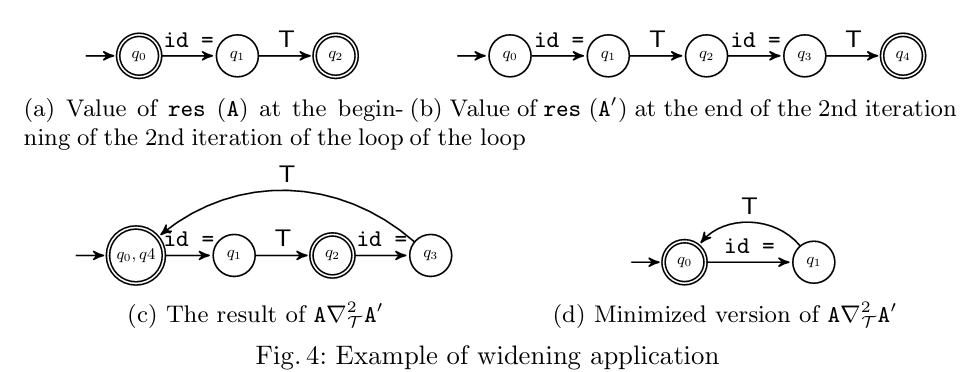
\includegraphics[width=\textwidth]{images/tarsis-widening.png}\hfill
\end{figure}